\section{Napotkane problemy}
Podczas tworzenia aplikacji zrezygnowaliśmy z Kubernetesa oraz Azure Kubernetes Service, koszty okazały się nieproporcjonalne do obecnego stanu i liczby użytkowników aplikacji. Aplikacja jest obecnie oparta wyłącznie na kontenerach dockerowych oraz innych modułach platformy Azure.

Kolejnym problemem napotkanym podczas tworzenia naszej pracy, były lokalne modele LLM, często bez odpowiedniej konfiguracji karty graficznej z kontenerem, operacje modelu były wykonywane wyłącznie na procesorze, spowodowało to bardzo duże opóźnienia w otrzymaniu jakiej koliwek odpowiedzi na wysłany prompt przez model językowy.

Dużym problemem okazały się rownież koszty utrzymania infrastruktury na środowisku deweloperskim, naszym budżetem na projket było około 200 złotych, jednak analizując prognozę kosztów w Azurze nasz budżet szybko został przekroczony. Największy koszt wygenerowały instancje kontenerów dockerowych działające w chmurze. 

\begin{figure}[h]
    \centering
    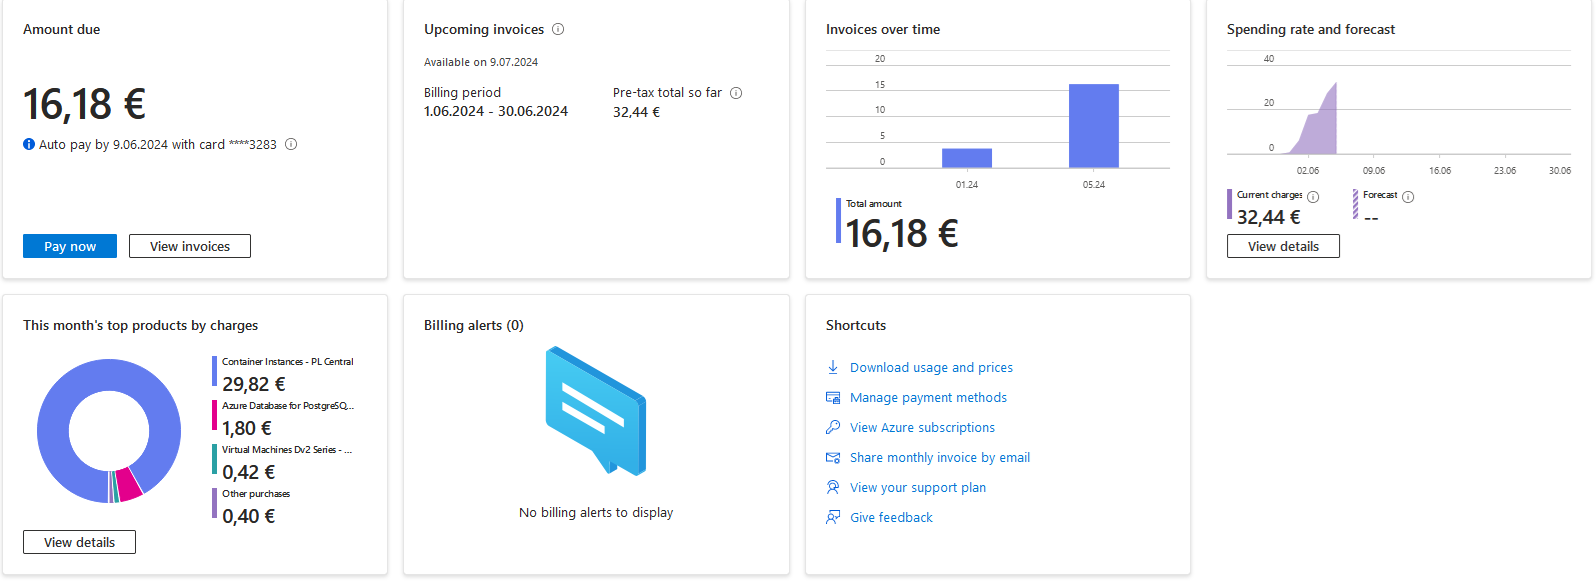
\includegraphics[width=1\textwidth]{Obrazy/costs.png}
    \caption{Prognoza kosztów na platformie Azure}
    \label{fig:my_label}
\end{figure}

\begin{figure}[h]
    \centering
    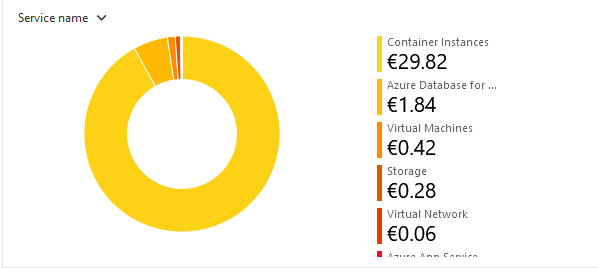
\includegraphics[width=1\textwidth]{Obrazy/costs3.png}
    \caption{Dokładna analiza kosztów z podziałem na moduły}
    \label{fig:my_label}
\end{figure}


\section{Rozwój}

\subsection{Plany na przyszłość}
Wraz z rozwojem aplikacji oraz przyrostu jej popularności i stabilności, niezbędne staje się przemyślenie kierunków jej dalszego rozwoju. Kluczowym aspektem, który planujemy wprowadzić, jest model biznesowy oparty o subskrypcję. Taki model przynosi wiele korzyści zarówno dla użytkowników, jak i dla nas jako deweloperów, oferując stabilne źródło przychodów oraz możliwość ciągłego rozwijania i ulepszania naszego produktu oraz utrzymania kosztów związanych z architekturą aplikacji.

Wprowadzenie modelu subskrypcyjnego pozwoli na regularne aktualizacje funkcjonalności oraz utrzymanie wysokiego poziomu wsparcia technicznego. Użytkownicy, subskrybując naszą usługę, będą mieli stały dostęp do najnowszych ulepszeń i dodatków, co zwiększy ich zaangażowanie. Model ten umożliwia również lepsze dostosowanie funkcji aplikacji do oczekiwań i potrzeb oraz pozwoli na pokrycie opłat związanych z infrastrukturą w chmurze.

Planujemy również rozszerzenie naszej oferty o nowe funkcje, które będą dostępne wyłącznie dla subskrybentów, takie jak zaawansowane analizy danych, personalizacja interfejsu czy specjalne opcje konfiguracyjne. Rozważamy także wprowadzenie różnych poziomów subskrypcji, co pozwoli użytkownikom wybrać plan najlepiej dopasowany do ich indywidualnych potrzeb i możliwości finansowych.